% !TEX root = ../paper.tex
%%
%%    THIS FILE IS NOT USED!
%%
%%    The Methods section has been merged with the Results section, now titled "Case Study."
%%

\section{Case Study}

Our case study used the Qt project review history from the Gerrit code review tool provided by Hamasaki et. al. \cite{Hamasaki2013}. Qt project is a large open source project composed of numerous small subsystems. We selected the most active subproject, which is called \texttt{qtbase}.
From this project, we used the review history before June 13\textsuperscript{th}, 2012, which has 6,605 changes and 72,484 comments in its Gerrit code review system.


% where we got the data
%We used the review data sets of the Qt project collected by Hamasaki et al\cite{Hamasaki2013}.
%Only reviews in the master branch of \texttt{qtbase} project are considered,
%as it is the most active branch.

% quick structure
%\pick{This already explain in background :D}
%Each change includes a \emph{commit message} which describes what is changed.
%After a change is submitted to Gerrit, reviewers can give scores to it.
%The scores will determine whether the change will be accepted or not.
%Reviewers can also add comments to the change, which may optionally be added to a specific line of code inside a changed file.
%Majority of the comments are automatically generated by Gerrit and do not contain any user-written text.

% overview
%In our classification method,
%all commit messages and comments that are human-written are converted into vectors using tf--idf algorithm.
%Few comments are sampled and then classified manually for use in training and validation.
%A model is created from these training data, from which useful comments can automatically be identified.
%This process is illustrated in Fig.\ref{fig:overview}.
%



\subsection{Data Preparation}
We used commit messages and comments in the dataset. Before classifying the usefulness of comments, we first processed the commit message and comments as follows: 

\subsubsection{Automatically generated messages removal}
In Gerrit, the comments are composed of comment messages from reviewers and automated messages. These automatic messages are generated by Gerrit and the integration system to record activities. For example, \textit{'Upload patch set 1.'}, \textit{'Change has been successfully cherry-picked to the staging branch as ...'}. Since these messages are generally recored keeping, they are not substantially relevant to the proposed changes and do not directly impact software quality\cite{Mcintosh} and hence are useless by our definition. In practice they are not considered in code review. They are easily determined as useless by our method and would artificially improve our classification performance. We identified these automatic messages using regular expressions and selecting frequently appeared patterns of messages.  


%The commit messages and all comment texts are converted into vectors as part of the preparation step.
%Fig. \ref{fig:preprocess} illustrates the overview of this step.
%We wrote scripts in Ruby language to perform these tasks.

%\begin{figure}[h]
%\centering
%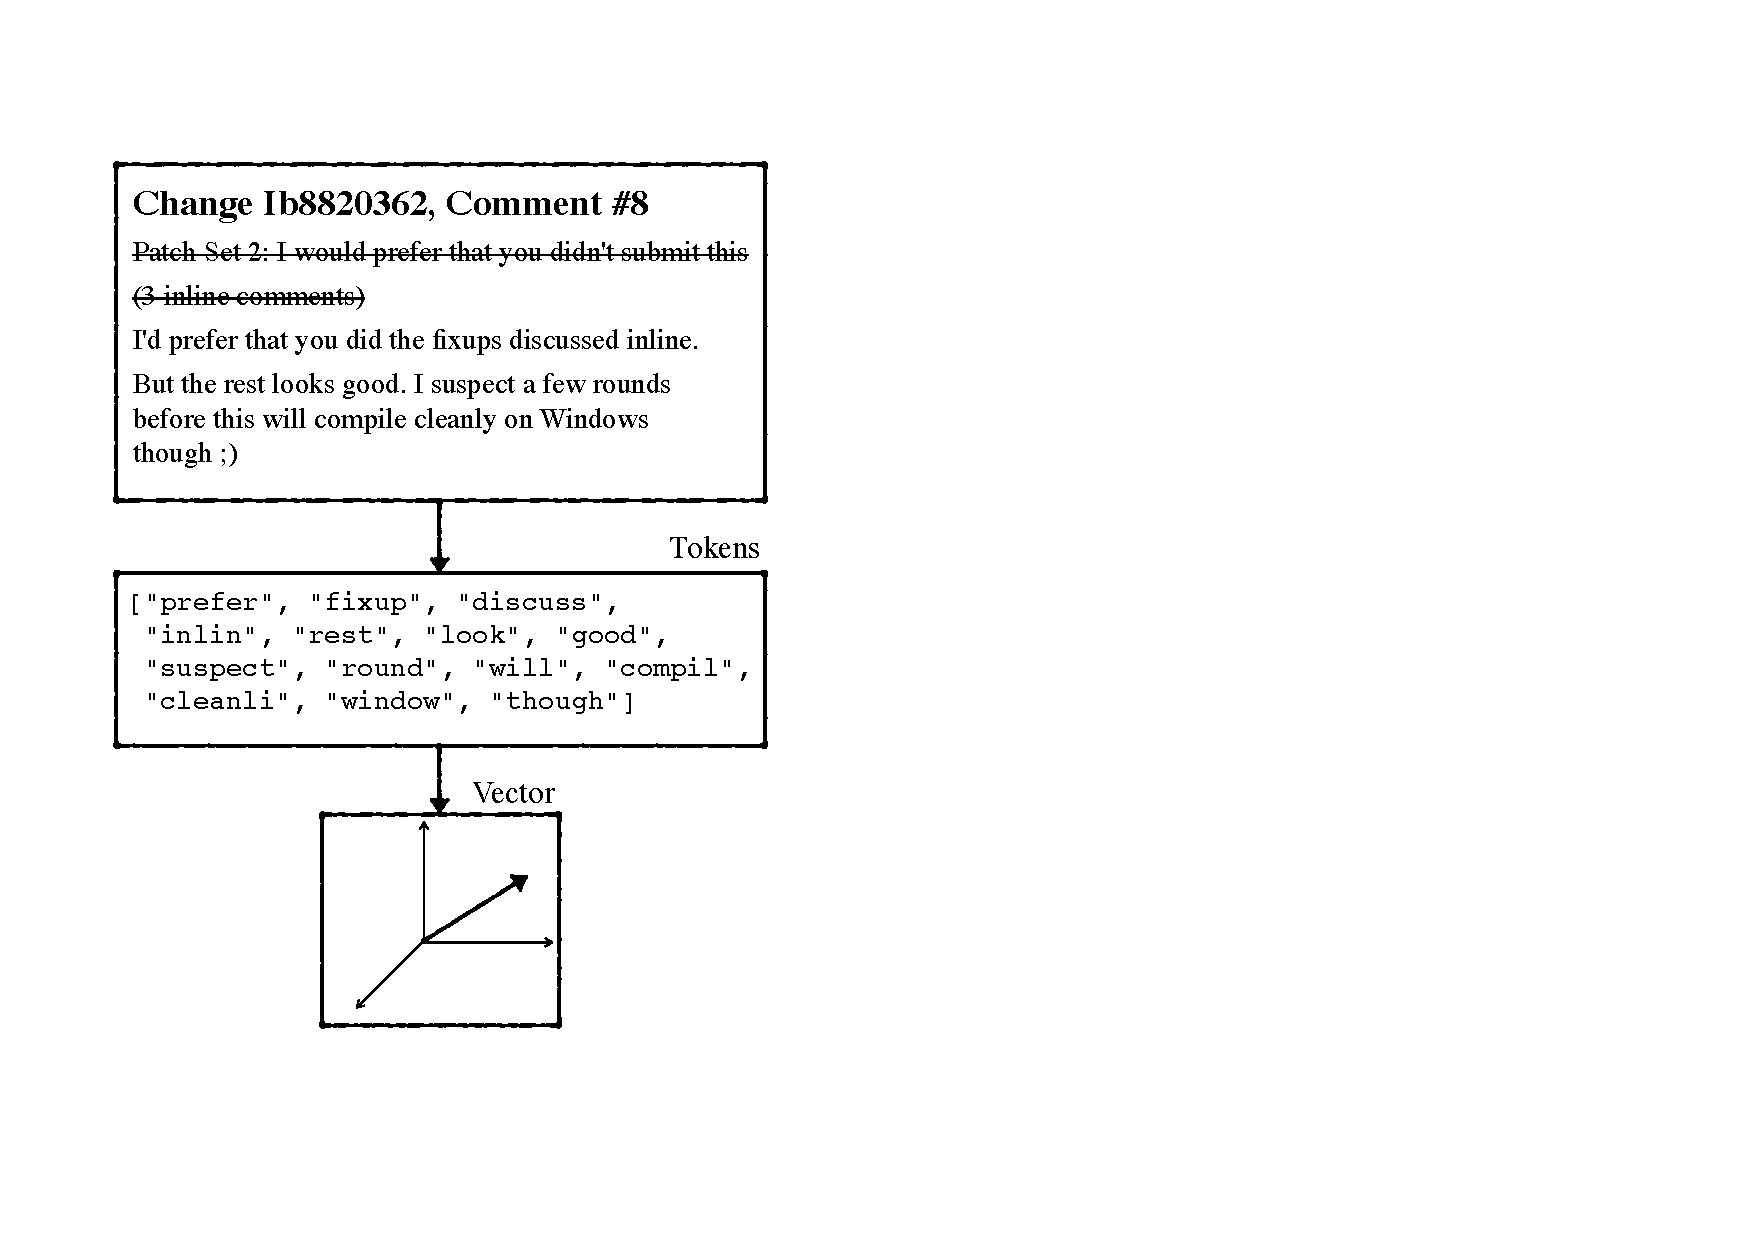
\includegraphics[width=3in]{preprocess}
%\caption{The data preparation process.
%Automatically generated texts are removed, remaining text is tokenized, stop words are removed, remaining tokens are stemmed,
%and are converted into a vector.}
%\label{fig:preprocess}
%\end{figure}



%\subsubsection{Removal of automatically generated text}
%
%First, all comments by the Gerrit system, \emph{Qt Sanity Bot}, and \emph{Qt Continuous Integration System} are skipped.
%
%% conversion into vector, wow
%Next, we looked for common patterns that appeared in the comments, because it is very likely that they are automatically generated.
%This is accomplished by splitting texts into lines, and for each line, searching for words that can be found in the English wordlist\footnote{The wordlist found in \texttt{/usr/share/dict/words} from Ubuntu Linux distribution is used.}.
%This effectively removed the ID numbers and other non-generic terms.
%
%Next, the lines that appears most frequently are identified.
%From these lines, we then constructed the regular expression patterns,
%and finally, these patterns are used to filter out automatically generated text from our data.



\subsubsection{Data Preprocessing}
 As is customary for VSM processing we extracted semantic words from commit messages and comment messages before converting to vector. For each message, we removed all punctuation signs, digits, and common words (e.g. a, an, the) using Google stop word list\footnote{Available at \url{http://meta.wikimedia.org/wiki/Stop_word_list/google_stop_word_list#English}}. We then used Porter stemming algorithm to remove the commoner morphological and inflexional endings from words in English.
 


%After the automatically generated messages are removed, we extracted the words in each document into a list of tokens by searching for alphanumeric characters including apostrophes.
%Stop words from the Google stop word list\footnote{Available at \url{http://meta.wikimedia.org/wiki/Stop_word_list/google_stop_word_list#English}} are then removed.
%The stemming is performed on remaining tokens using Porter stemming algorithm.
%The remaining words are then combined to form a corpus of all used words.



%\subsubsection{Conversion into vector}
%
%Finally, the tf--idf algorithm is used to convert each document into a vector.

\subsubsection{Ground-Truth Data Preparation}
To prepare ground-truth data, a team of three experienced developers independently read comments and manually assessed them useful or useless. The assessors were asked to answer for each comment the question ``Does this comment technically contribute to its proposed change?''. Then, the assessors cast their vote as \texttt{YES} if the comment is likely to useful and \texttt{No} if the comment is likely to useless.  Comments with three \texttt{YES} votes are classified as \textbf{useful} comments and comments with three \texttt{NO} votes are \textbf{useless}. Comments lacking unanimity i.e. one or two \texttt{YES} votes are deemed \textbf{unclear} and not confidently useful or useless. 

\subsection{Research Questions}
To validate our approach, we addressed the following research questions:

\dan{Why is this a separate section? Either the actual results should deb discussed here or this should be integrated into the results section.}

\noindent \textbf{RQ1: Is semantic similarity a good indicator of MCR comment usefulness?}\\
\indent To answer this question, we randomly sampled 320 comments from our data set and manually identified usefulness as described in previous subsection. Then, we used these comments for both the training and test data set for our approach to determine its effectiveness. We also determined the effectiveness of our approach using bootstrapping cross validation. We randomly selected 90\% of 320 comments for training set and 10\% for the validation set.
The performance on the 10\% was measured using precision, recall and F-measure as described in Equation \ref{eq:fmeasure}. We repeated this validation for 300 times to estimate the mean and variance of the performance.

\dan{What what the effort in person-hours for this?}

Since our models do not include unclear type of comments, we defined them as negative condition i.e useless comments in case of useful classification (when using $\Theta(c,S_T,D_T)$ model) and useful comments in case of useless classification (when using $\Omega(c,S'_T,D'_T)$ model).
\dan{I thought we changed this! It would be bad if we didn't. Let me know what the actual situation is here.}

%We sampled 320 comments from the data set.
%These samples are then classified as either useful (that is, technically contributing to the software) or not useful.
%This task is carried out by three people who worked independently.
%
%Each comment is then scored based on the number of positive answers.
%For example, a comment with a score of 3 means that all three people said that it is useful,
%while a comment with a score of 0 means that none of us marked it as useful.


\noindent \textbf{RQ2: Do code reviewers intensively discuss on the proposed changes?}\\
\indent To answer this question, we estimated similarity and dissimilarity thresholds using comments from RQ1 for training set. We then used these thresholds to classify the rest of comments. A statical analysis was performed to understand the impact of useful discussion to software quality.
\dan{results?}

\noindent \textbf{RQ3:  Is semantic similarity classification cost-efficient, assur- able, and scalable?}\\
\indent
\dan{results?}


%\subsection{Training Data}



%The score of a comment can be defined as:

%\begin{align*}
%Score_i & = \sum_{\text{reviewer } r} Review(r, i). \\
%Review(r, i) & = \begin{cases}
%	1 & \text{if } r \text{ says that the comment } i \text{ is useful,} \\
%	0 & \text{otherwise.}
%\end{cases}
%\end{align*}



%\pick{I re-wrote of these, hope I don't miss something ;)}
%\subsection{Model Generation and Validation}
%
%% the metrics
%For each comment, we computed similarity and dissimilarity metrics
%between the comment text and the corresponding commit message.
%We chose cosine similarity and euclidean distance as the metrics to use in model generation.
%
%\begin{figure}[h]
%\centering
%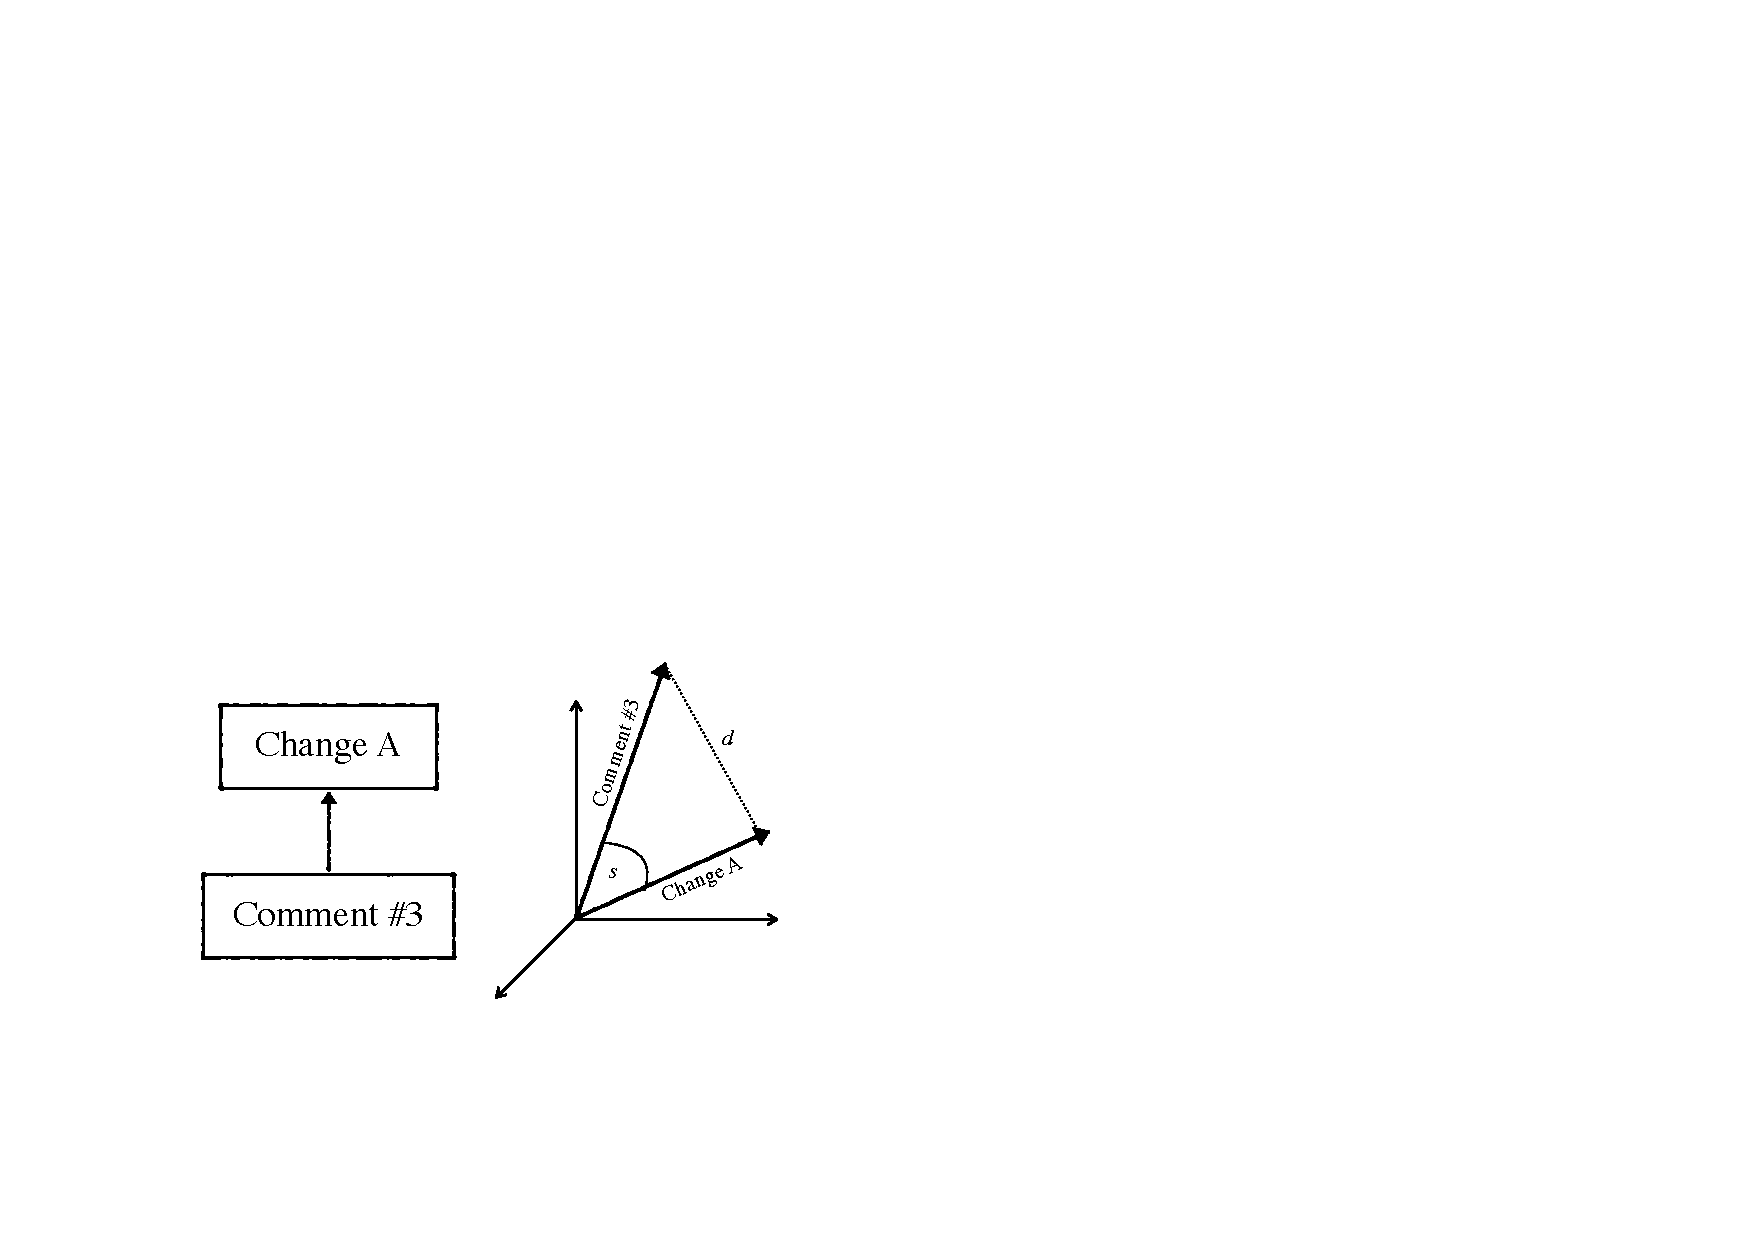
\includegraphics[width=3in]{vector}
%\caption{The similarity and distance metric that is being used.}
%\label{fig:vector}
%\end{figure}
%
%% assumptions in categorization
%The model is based on two assumptions: that useful comments will have a $similarity \geq A \text{ and } distance \leq B$,
%and that comments that are not useful will have a $ similarity \leq C \text{ and } distance \geq D$,
%where $A$, $B$, $C$, and $D$ are some constant.\footnote{We also tried using the `or' operator, and found that using `and' produces better result.}
%
%% finding parameters
%To find these parameters, a brute-force approach is used.
%This is possible because the set of $similarity$ and $distance$ values are discrete.
%Each possible value of $A$, $B$, $C$, and $D$ are evaluated to find the constant that returns the maximum F$_1$ score.
%
%% validation
%To validate our model, we randomly split the data into 10 parts.
%9 parts are used for training, and 1 part for validation.
%This process is repeated 300 times. % while I sleep
%The values of precision, recall, F$_1$ score, and accuracy are recorded and then averaged
%to give the overall performance of our model.

